% Version-specific figures. main.tex (v1) inputs figs_v1.tex; main_v2.tex inputs figs_v2.tex.
% The sections call \FigureEncSeeds (column width, in sec:encoder) and \FigureLLM (text width, in sec:llm).
% v2: the same numbers, re-drawn for print by clarity/paper_figures.py (vector PDF, serif type).

\newcommand{\FigureEncSeeds}{%
\begin{figure}[t]
\centering
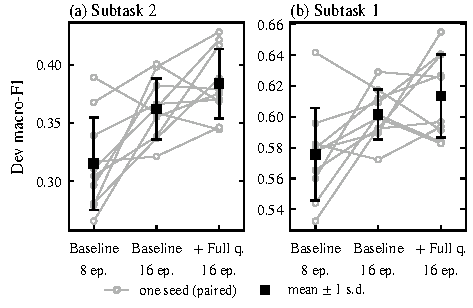
\includegraphics[width=\columnwidth]{figures/v2/fig_deberta_seeds.pdf}
\caption{Single DeBERTa-v3-large models on dev for the three configurations: (a)~\Stwo{} multi-reference macro-F1, (b)~\Sone{} macro-F1. Open circles joined by thin lines are individual seeds, paired across configurations; filled squares are the mean over the 10 seeds, with error bars of $\pm 1$ standard deviation.}
\label{fig:enc-seeds}
\end{figure}}

\newcommand{\FigureLLM}{%
\begin{figure*}[t]
\centering
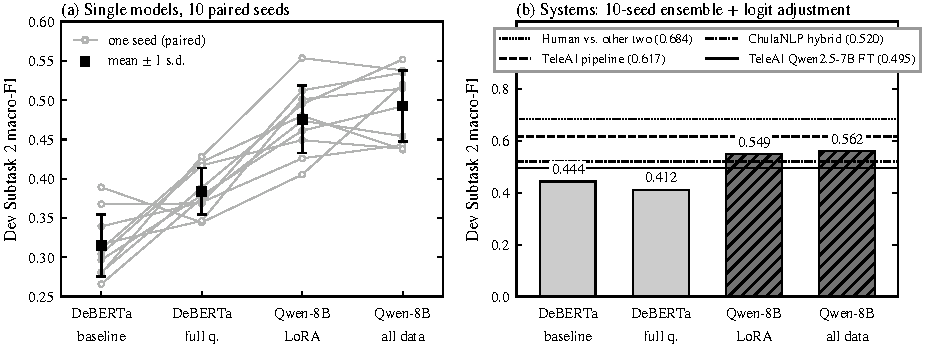
\includegraphics[width=\textwidth]{figures/v2/fig_qwen_vs_deberta.pdf}
\caption{Dev \Stwo{} multi-reference macro-F1 of the DeBERTa-v3-large baseline, DeBERTa with the full question and 16 epochs, Qwen3-8B-Base with LoRA on the same input (3 epochs), and Qwen trained on all of train. (a)~Single models on 10 paired seeds: open circles joined by thin lines are individual seeds; filled squares are means with $\pm 1$ standard deviation. (b)~The corresponding 10-seed systems (ensemble + logit adjustment, $\tau$ by nested CV; bar height is the mean over 10 CV splits), with published dev results as horizontal lines: TeleAI's multi-call pipeline (0.617) and fine-tuned Qwen2.5-7B (0.495) \citep{shi-etal-2026-teleai}, ChulaNLP's DeBERTa top-5 + Kimi-K2 pipeline (0.52) \citep{peerachaidecho-rutherford-2026-chulanlp}, and a human annotator scored against the other two (0.684).}
\label{fig:llm}
\end{figure*}}
